\chapter{NLG Tasks}\label{chap:tasks}
Transforming non-linguistic data into grammatically correct sentences in a given language seems like a rather complicated problem. Therefore it is convenient to divide the initial problem into smaller tasks, which are easier to solve. This task structure is described by \cite{reiter1997building} and it is widely used to cover every challenge a fundamental NLG problem should deal with:
\begin{itemize}
	\item Content determination
	\item Discourse planning
	\item Sentence aggregation
	\item Lexicalization
	\item Referring expression generation
	\item Linguistic realisation
\end{itemize}

In this section we will discuss every task mentioned above. Note that approaches, which will be described later, may change this structure: there might be just a few changes by combining multiple steps and processing them simultaneously or the structure may be completely decomposed. Moreover, using data-driven methods is dominant approach and can be utilized across every task of the NLG. Their usage will be omitted in this section and further closely discussed in \autoref{chap:approaches} taking the uniqueness and dissimilarity of this approach into consideration.

The reason we describe every task individually is to highlight challenges that will arise along the way of creating the NLG system. Understanding these tasks is a crucial aspect to produce a well-built software regardless of the choice of the approach. To illustrate the problems we state numerous simple examples that should ease the process of fully recognizing the extent of issues related to each task.

\section{Content determination}
The goal of this task is to decide what information from input data should be included in the text. Usually the range of the input data is significantly larger than the amount of information we would actually transfer to the user. Naturally, this task is heavily influenced by the specifications of the assignment, namely domain, intention of the text and target audience. Consider the problem of creating a medical report from a complete blood count for a patient to read. This domain requires data preprocessing to recognize negative indicators from values contained in test results. In addition, a doctor or expert is needed to assist in order to interpret values correctly and set rules on how to identify diagnosis. The goal of the text is to describe the diagnosis in an understandable way and therefore using Latin or overly technical terminology should be avoided. However, if we take the doctor as a target audience, we now want to use the as precise expert language as possible and probably change the content to present segments of the test results and not just the overall diagnosis to enable the doctor to better interpret marginal symptoms or flag values.

The result of the content determination is usually outputted as a set of preverbal messages, carrying semantic meaning of the statement. To carry all the information an implementation that can describe abstract concepts such relations between statements, entities or conditions is needed. This sub-task of creating suitable representation is usually domain-dependent. Since the important semantic information is mapped into some formal language, there is no need for (human) language to be specified, and therefore this task is language-independent. Concrete examples of formal representation language used to store these semantic attributes are for instance logical language, attribute-value matrices or graphs.

Example of the result of possible content determination is shown below in \figref{cd}, where we would like to choose the content to report one simple message: a goal being scored in a football domain. We have two related (3) sets of attribute-value pairs: (1) is about a player and (2) contains goal statistics. Obviously some information in tables (1) and (2) are too specific (e.g. height of the player) for the message to convey and therefore redundant. Bold attribute-value pairs are highlighted as the ones to be present in the final text, creating preverbal message (4) in pseudocode, which is an output of content determination task. After performing the remaining NLG tasks possible result could look like (5). 

\begin{figure}[h]
	\centerline{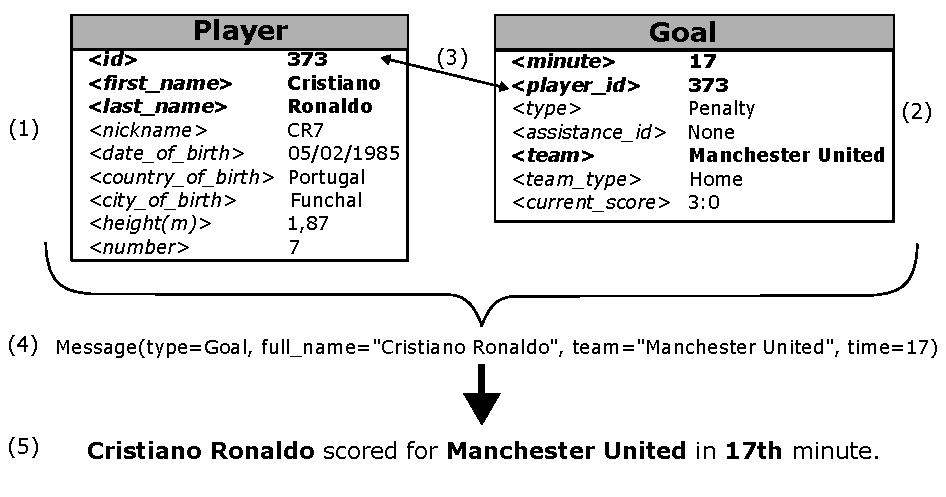
\includegraphics[width=0.9\textwidth]{../img/content_determination.pdf}}
	\caption{Process of content determination}
	\label{fig:cd}
\end{figure}

\section{Discourse planning}
Previous part determines what messages will be transmitted to the reader and this part resolves the issue of the order in which the information is presented. This process is also referred to as text or document structuring. Selecting the right sequence of messages is crucial for text to accomplish its goal. Similarly we structure academic texts to logically ordered paragraphs, which present the topic in a way as understandable as possible for the reader to gain knowledge.

Similarly to content determination this task is highly domain-dependent as we have to know how to order messages. For instance, a medical report (as an example mentioned earlier) would likely display diagnoses and order decreasingly by how dangerous and life threatening they are. On the other hand, a report from a business meeting could start with a brief overview of achievements and goals and then with issues that were discussed ordered chronologically to allow the reader to follow the course of the meeting.

Human brain orders information to be conveyed in a speech intuitively, but the process as an algorithm itself is not quite trivial. Most of common method is to create rules based on the specific domain since the suitable structure heavily relies on the domain. Some researchers suggest using machine learning techniques for creating a  uniform algorithm independent of the domain as seen in \cite{dimitromanolaki2003learning}.

Form of the output of discourse planning can differ. One possible option as described by \cite{reiter1997building} is a tree structure. Leaves of the trees are messages and inner nodes describe specifics of their function in a sentence. This may seem like an unnecessary complicated solution when clustering messages to be said in one sentence can be just an array of messages. The benefit of the tree structure is the amount of information we can store along the messages including constraints under which the message can be said, relations between them and their overall structure.

\section{Sentence Aggregation}
The cardinality of the relation message and sentence is rarely one-to-one. Usually multiple messages are formed into one sentence. This process is called sentence aggregation and it is fundamental for generating text that is readable and flows well. To clarify we provide set of verbal messages:
\begin{enumerate}
	\item \emph{Peter bought an apple.}\label{sa-one}
	\item \emph{Peter bought a banana.}\label{sa-two}
	\item \emph{Anne did not buy anything.}\label{sa-three}	
\end{enumerate}

This set of sentences is clearly non-optimal and can be aggregated in two steps as follows:\footnote{\label{footnote-opt}Naturally, no such concept as "optimal" sentence exists. The optimum in this case is to express the information in a sentence that would likely occur in a spoken human language and also would appear fluid and natural.}
\begin{enumerate}[resume]
	\item \emph{Peter bought an apple and a banana. Anne did not buy anything.}\label{sa-four}
	\item \emph{Peter bought an apple and a banana, whereas Anne did not buy anything.}\label{sa-five}	
\end{enumerate}

We can notice two types of aggregation leading to the optimal sentence (\ref{sa-five}). Aggregation of:
\begin{itemize}
	\item \textbf{constituents} - Constituents that have equal syntactic importance can be aggregated using suitable coordinating conjunctions expressing their relation. Take example sentences (\ref{sa-one}) and (\ref{sa-two}). \emph{Apple} and \emph{banana} are both items \emph{Peter} bought so their semantic meaning is identical. Therefore they can be aggregated via cumulative conjunction \emph{and} creating a new noun phrase in the result sentence (\ref{sa-four}) \emph{an apple and a banana}. Another example of cumulative conjunctions is \emph{both ... and} or \emph{as well as}.
	\item \textbf{sentences} - Sentences can be aggregated as well using coordinators as seen in the result sentence, which was created by inserting an adversative conjunction in between sentences in example (\ref{sa-four}) to express opposition. This contrast can be expressed by other words like \emph{but}, \emph{yet}, \emph{while}, etc. More relations can be expressed when aggregating sentences using another kinds of coordinating conjunctions: \emph{alternative} (\emph{or}, \emph{either ...or}, \emph{nor}) to express two or more alternatives and \emph{illative} (\emph{for}, \emph{so}) to express interference or consequence.
\end{itemize}

One more type of aggregation can occur based on explicit hand-crafted domain-based rules. Take these three preverbal messages from football domain reporting a goal, which are similar to the one as used in \figref{cd}-(4) (Manchester United shortened to MU):
\begin{enumerate}[resume]
	\item \emph{(type=Goal, full\_name="Cristiano Ronaldo", team = "MU", time = 4)}\label{sa-six}	
	\item \emph{(type=Goal, full\_name="Cristiano Ronaldo", team = "MU", time = 8)}\label{sa-seven}
	\item \emph{(type=Goal, full\_name="Cristiano Ronaldo", team = "MU", time = 14)}\label{sa-eight}	
\end{enumerate}

Surely realising messages (\ref{sa-six}), (\ref{sa-seven}) and (\ref{sa-eight}) as three different sentences would not create fluid and natural results as sentences would vary only in time of the goal. Since three goals in football form a so called hat-trick we could aggregate messages in one sentence:
\begin{center}
	\emph{Cristiano Ronaldo completes hat-trick for MU in under 15 minutes.}
\end{center}

This aggregation realises the messages (\ref{sa-six}, \ref{sa-seven}, \ref{sa-eight}) beautifully as the result is well-formed and natural. Notice that the aggregation happened also in expressing the time of the goals: instead of mentioning three different timestamps the time is summarised as "under 15 minutes" highlighting the fact that this rare figure was achieved in a short amount of time. As described in the previous section, domain knowledge is necessary to decide what is "long", "short" or "average" (and therefore not worth mentioning) amount of time for an event to happen.

Note that these aggregations are simple for humans, but to perform them in a NLG we need some semantic knowledge and relations of the sentences (or constituents). The easiest approach is to define domain-specific constraints when to perform aggregation. Defining complex domain-independent rules and universal representation of relations is rather a difficult task and nowadays often solved using data-driven methods, which are described later in \autoref{chap:approaches}. 

Furthermore, the idea that the more aggregations we perform the better the final text is wrong. Sometimes slowing down the flow of information by fracturing the message into smaller individual sentences is useful in order to produce more understandable text. Overloading sentences can often result in less fluency as the more information is conveyed in one sentence the harder it is for a reader to follow. \cite{barzilay2006aggregation} are perceiving this as a linear programming problem where similarity is classified for each pair of database entries. Using this similarity, transitivity and global constraints (e.g. maximum number of aggregation across the document) they find an optimal solution.   

\section{Lexicalization}
After performing discourse planning and sentence aggregation the preverbal messages are in a correct order and they contain suitably aggregated information. Goal of this task is to create mapping from these messages to specific expressions in a given human language. This task is the first that is language-dependent. There are two main problems associated with lexicalization. Firstly, the amount of combinations of how to narrate a message is enormous, only restricted to those that fit into the given context. And secondly, transformation of concept into a word (or more words) is very abstract and interferes with many layers of the language (semantics, phonetics and pragmatics) and therefore choosing a suitable expression is rather difficult. This transformation is not even easy for humans. Imagine an essay contest in grammar school with a given topic of the essay. If the transformation was easy and had only one solution, the contest would not exist as essays would be identical. In fact, the perspective and overall understanding of the topic, style of describing one’s point of view and finally even choosing words to present the idea is partly what distinguishes us as people. 

Another factor is the target audience and the overall goal of the language. If the target audience is educated on the matter then using adequate technical terminology is reasonable. Contrastingly, for low-skilled readers all terminology must be explained in an easy way and the content of the text should be more about overall ideas rather than about specific concepts. 

Trivial approach to this task is to hand-craft pairings of a word or a whole phrase and a concept in a message. This solution results in monotonic outputs as the aspect of choice is missing. Slight improvement would be to add more semantically similar options for each item. However, this can cause problems. First of them is how to decide, which possibility is the best. Second is the possible non-viable combinations of words together. One example, that may be not visible on the first glance, is generation of adjectives interpreting numbers. For example, take a person with height 185 cm. If it was a man, the height is "average", while a woman could be described as "tall". Therefore semantic background and suitable comparison need to be taken into account. What is more, combinations of chosen phrases may result in non-realisable or simply weird expressions. 

Due to the vagueness and coherence of the process, NLG systems combine lexicalization, REG and linguistic realisation under one operation called surface realisation or tactical part of the process.  

\section{Referring expression generation}
Referring expression generation (REG) is a process, when you choose words to express domain entities or other constituents of the message. Naturally, utilising one noun phrase for one specific entity, which is used more than once in a short amount of text, results in less readable and fluid text. On the contrary, there is a limit to how many such expressions we can generate since a reader needs to identify the entity correctly. Ambiguity is a highly unwanted effect since the information that needs to be conveyed may differ from its actual language semantic meaning.

To fully understand the challenges and also possible solutions for REG here is an example of sentence where we would like to lexicalize its subject represented as an entity in pseudocode:
\begin{center}
\emph{(entity=Country, name=”Czech Republic”) has a population of 10,3 million.}
\end{center}
This particular country can be lexically expressed in this sentence for example as:
\begin{enumerate}
	\item \emph{Czech Republic} \label{reg-1}
	\item \emph{Czechia} \label{reg-2}
	\item \emph{Country nicknamed “The heart of Europe”} \label{reg-3}
	\item \emph{Bohemia, Moravia and Czech Silesia} \label{reg-4}
	\item \emph{Country in the central Europe} \label{reg-5}
	\item \emph{Country which borders Germany, Poland, Slovakia and Austria} \label{reg-6}
	\item \emph{Beautiful rustic country in the heart of Europe} \label{reg-7}
	\item \emph{It} \label{reg-8}
	\item \emph{This country} \label{reg-9}
\end{enumerate}
Notice the linguistic techniques we used to express this subject:
\begin{itemize}
	\item \textbf{Entity name} - Using the name of the entity is a trivial solution and works fine as seen example (\ref{reg-1}).
	\item \textbf{Synonyms} - Using a synonym or a different name having the identical semantic meaning for the entity as shown in example (\ref{reg-2}) and (\ref{reg-3}). 
	\item \textbf{Descriptive transcription}  - using the knowledge of physical appearance, characteristics or its location we can describe an entity without any need of using its initial name. Examples (\ref{reg-5}), (\ref{reg-6}) and (\ref{reg-7}) are all using the location in Europe. Although expression (\ref{reg-6}) identifies Czechia unambiguously, the description of the location may be too specific for a less-educated reader (or possibly for a reader living outside of Europe), who has no idea where Germany is. The information that the country is situated in Europe is then sufficient. Therefore the target reader, his knowledge about a topic and also the purpose of the text are important even in this task. This technique is also prone to ambiguity as seen in example (\ref{reg-5}): reader should already know what country is described in the text to use this expression since more countries can be characterised as “central European”.
	\item \textbf{Definite descriptions} - The expression can be enriched by adding valid adjectives, adverbs or other linguistic structures to further specify the object as seen in example (\ref{reg-7}) where adjectives rustic and beautiful describe the country even a little bit more creating enriched and complex noun phrase.
	\item \textbf{Pronouns} - In a human language pronouns are often used to represent entities (e.g. “I have seen him.” or examples (\ref{reg-8}), (\ref{reg-9})). Using pronouns correctly can help to improve readability of the text and also minimise the obvious flags of computer-generated text. The main obstacle to overcome is when to use pronouns. Sometimes usage of a pronoun can arise from context, sometimes if there is absolutely certainty that everyone knows what the pronoun is referring to: those examples are hard to deal with and usually handled explicitly. Usual approach is to use pronoun if the entity was mentioned in a previous sentence under the condition the entity was the only constituent the pronoun could refer to.
\end{itemize}

How to approach REG depends also on repetition of the entities in the text and the final text variability. In a domain where identifying the entity unambiguously is primary (e.g. city in air travel) the usage of REG is even harmful. For instance, expressing "New York, USA" as "The city that never sleeps" in the air travel domain. To the contrary, expressing an entity identically multiple times in a short span of prosaic text eventuates in dull, plain and stereotypical language. 

\section{Linguistic realisation}
This task transforms every constituent to form a grammatically and syntactically well-built sentence. Example of a struggle when building even a simple noun phrase is:
\begin{enumerate}
	\item \emph{(entity=Animal, name =”dog”, count=1) $\rightarrow$ one dog} \label{lr-1}
	\item \emph{(entity=Animal, name=”dog”, count=23) $\rightarrow$ 23 dogs} \label{lr-2}
	\item \emph{(entity=Animal, name=”mouse”, count=2) $\rightarrow$ two mice} \label{lr-3}
	\item \emph{(entity=Animal, name=”fish”, count=1000) $\rightarrow$ thousand fish} \label{lr-4}
\end{enumerate}

Trivial and also naive solution for this simple noun phrase building can be to append morpheme “s” to the name of the animal if the count is more than one. As you can see in example (\ref{lr-3}) and (\ref{lr-4}) this solution can work only for animals that have regular plurals. In addition, the count itself is recommended to be expressed by a word and not by numeral if the number is either a small integer (1-10) as seen in the comparison of  examples (\ref{lr-1}) and (\ref{lr-2}). Same rule applies as well for a well-known rounded number (hundred, thousand, billion, etc.) shown in (\ref{lr-4}).

One, so far omitted important, aspect is the principles of morphology and syntax of the language. Concept of appending morpheme "s" to express plural might not be so easily transferable into different languages. In Slavic languages morphemes to express plural differ and also can be infixed, meaning they could be inserted into the word stem instead of using a suffix. In Czech, a word for dog is \emph{pes}. Then realising their number would look like: \emph{1 pes, 2 psi, 5 psů}. To further complicate the situation, Slavic languages are fusional. That means a single morpheme carries multiple grammatical, syntactic or semantic meanings. In Czech, agreement between the grammatical case and the noun is resolved as well with an infix morpheme. Here are three examples in Czech using different grammatical cases along with translation from English:

\begin{itemize}
	\item (case: nominative) \emph{two \textbf{dogs}	$\rightarrow$ dva \textbf{psi}}
	\item (case: genitive) 	\emph{without two \textbf{dogs}  $\rightarrow$ bez dvou \textbf{psů}}
	\item (case: instrumental) \emph{with two \textbf{dogs} 	$\rightarrow$ s dvěma \textbf{psy}}
\end{itemize}

Notice that not only the noun, but the word for number 2 (\emph{dva}) as well are subject to the linguistic transformation as the infix morpheme carries both the agreement with case and the plural. 

We have mentioned typology according to morphology (fusional language). Another type is analytic languages (e.g. Vietnamese), where every single word is exactly one morpheme. Lastly, the complete opposite is polysynthetic languages (e.g. Inuit languages), where one word is constructed by combining plenty of morphemes representing a whole sentence. In central Nunavut Inuktitut \emph{Tusaatsiarunnanngittualuujunga} means \emph{I cannot hear very well}. 

The extent of language influence is huge even in the semantic part as well. To demonstrate, imagine generating a sentence, in which the action will happen in the future. This may seem like a trivial problem in English since we may just use the word "will" (or other modals). However, English, unlike Romance languages (French, Spanish, Italian and more) does not have future grammatical tense. Some languages are even tenseless, e.g. Tokelauan spoken in American Samoa (Polynesia). This section just illustrated the need for the knowledge and principles of the language during the linguistic realisation.  

Realisation has quite an extensive magnitude caused by the non-trivial goal of correctly morphologically and syntactically (as well as semantically) expressing each of the lexical items in the sentence. This process requires adding auxiliary words (prepositions, verbs, etc.), handling agreements, ordering,  inserting punctuation and other similar transformations all in order to present the language not only factually, but even grammatically right. Due to the complexity of the task multiple approaches exist. One of them is using templates. 

\textbf{Templates} are hand-crafted using fixed lexical items and attributes substituted in the template. Preverbal message (\ref{lr-t-1}) is assigned to a template (\ref{lr-t-2}) and three variables are then substituted with values creating the target sentence (\ref{lr-t-3}). 

\begin{enumerate}
	\item preverbal message $\rightarrow$ Message(type=Goal, full\_name = "Cristiano Ronaldo", team = "Manchester United", time = 17) \label{lr-t-1}
	\item template $\rightarrow$ \textbf{\$full\_name} \emph{scored for} \textbf{\$team} \emph{in} \textbf{\$minute}\emph{th} \emph{minute}. \label{lr-t-2}
	\item result $\rightarrow$ \textbf{Cristiano Ronaldo} \emph{scored for} \textbf{Manchester United} \emph{in} \textbf{17}\emph{th} \emph{minute}. \label{lr-t-3}
\end{enumerate}

The advantage of this approach is simplicity and prevention of grammatical errors considering that we have full control of what the fixed segments are and any unwanted error is highly improbable. The disadvantages prevail. First of all, applying templates could be only feasible in well-defined low-volume domains as entities must be have easy-to-text-interpretation. Another reason is that creating templates is time-consuming. And most importantly, the variation of the output is low as the immutable parts of the text generate very limited output. In addition, the template approach for more complicated languages tends to struggle, because the constituents usually depend on each other (e.g. agreement, auxiliary words, etc.) creating requirements that are hard to fulfil. 

However, templates are extremely practical when the target output is expected to be simple and 
rarely changing. Great example is generating spoken announcements in the transportation domain e.g. departures of flights on the airport, where the template could look like: \emph{The departure of flight number \$number from \$destination\_from to \$destination\_to will be slightly delayed. $\rightarrow$ The departure of flight number FD-2018 from Rome to Paris will be slightly delayed}. Results are admittedly blunt in terms of language richness, but they are factually correct, clear and easy to comprehend, which was the initial purpose.
     
Other approaches are more complicated in order to outperform templates in a range of expressions.  First of them is building a grammar for the natural language. This approach relies on thorough knowledge and examination of the language behaviour and principles offering domain-independent solutions that can be applied to a different NLG system performing linguistic realisation. The advantage of this approach is definitely the domain independence of the realiser as well as its variety in produced output. Disadvantage is that building such grammar is labour-expensive and the disability to select the best possible result. All generated sentences will be correct, but the choice, which one is the optimal one is beyond grammar's reach.

Secondly, data-driven (further described \autoref{chap:approaches})methods can be applied in this task too. However their usage can vary greatly. Both approaches above can be enhanced by these stochastic methods since we can reduce manual workload. Templates can be automatically extracted from training corpus (more about corpora in \autoref{chap:process}). Similarly, hand-crafted grammars can be created automatically from corpora. Also, linguistic approaches can be avoided by using these methods. However, fusing traditional linguistic approaches and the power of statistical approach can result in a well-performing system. For instance, using hand-crafted grammar in combination with stochastic methods to resolve the optimal-among-the-correct-ones issue.


